\section{Design}\label{sec:dsg}

  The PlantUML application was used to create all of the figures in this
  section, the color scheme and icons to define field and method visibility
  in class diagrams are given below in Table~\ref{tab:uml-vis}.

  \begin{table}[H]
    \centering
    \begin{tabular}{c c c}
      \toprule
      Icon for Field & Icon for Method & Visibility \\ [0.5ex]
      \midrule
      
\includegraphics{figures/design/field-private} & 
\includegraphics{figures/design/method-private} & Private \\
      
\includegraphics{figures/design/field-protected} & 
\includegraphics{figures/design/method-protected} & Protected \\
      
\includegraphics{figures/design/field-package-private} & 
\includegraphics{figures/design/method-package-private} & Package Private \\
      
\includegraphics{figures/design/field-public} & 
\includegraphics{figures/design/method-public} & Public \\
      \bottomrule
    \end{tabular}
    \caption{PlantUML Class Diagram Visibility}\label{tab:uml-vis}
  \end{table}

  % TODO describe how abstract and static are shown
  % TODO create a table with images showing how class diagram relationships are shown

  \subsection{Use Cases}\label{sec:dsg-use}

    % good example of use case in "Bootstrap grids day 2" http://www.bossable.com/577/mean-stack-bootstrap/

  \subsection{Classes}\label{sec:dsg-classes}

    The UML class diagrams for included in this section are a best guess of
    what the system as a whole will require. As much of the core of OpenDCS
    is a rewrite and adaptation of an existing system some of what will be
    required is known, but may change during implementation because of the
    different use cases that will be developed.

    Much of what will be required for the complete system was not documented
    during the design stage, there are many components that do not need to be
    available to test, verify, and validate the project requirements. For
    instance, classes for data acquisition components such as analog input
    channels, serial ports, and digital output channels, are not required and
    a test device can be developed that produces dummy data. The focus will
    really be placed on the key components such as application design and the
    classes that are responsible for communication among the services.

    % If for some reason I choose to do a write-up describing each class
    % consider using wrapfigure

    \subsubsection{Core Library}\label{sec:dsg-classes-core}

      \emph{DcsAbstractBuildable}

        \begin{figure}[H]
          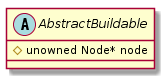
\includegraphics{figures/design/class/core/abstract-buildable}
        \end{figure}

      \emph{DcsAbstractConfig}

        \begin{figure}[H]
          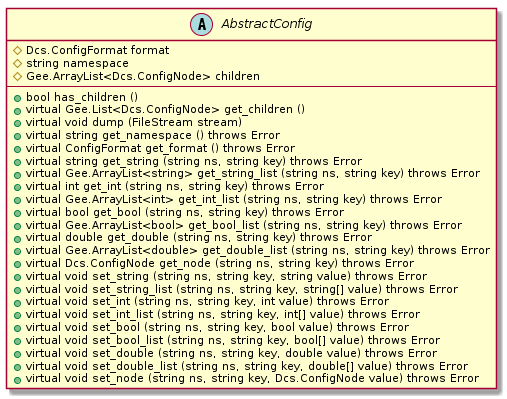
\includegraphics{figures/design/class/core/abstract-config}
        \end{figure}

      \emph{DcsAbstractContainer}

        \begin{figure}[H]
          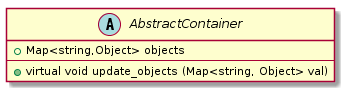
\includegraphics{figures/design/class/core/abstract-container}
        \end{figure}

      \emph{DcsAbstractObject}

        \begin{figure}[H]
          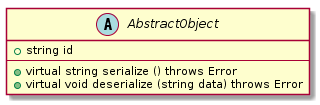
\includegraphics{figures/design/class/core/abstract-object}
        \end{figure}

      \emph{DcsApplication}

        \begin{figure}[H]
          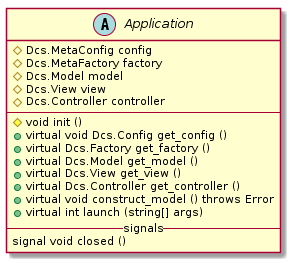
\includegraphics{figures/design/class/core/application}
        \end{figure}

      \emph{DcsBuidable}

        \begin{figure}[H]
          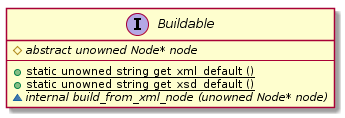
\includegraphics{figures/design/class/core/buildable}
        \end{figure}

      \emph{DcsConfigNode}

        \begin{figure}[H]
          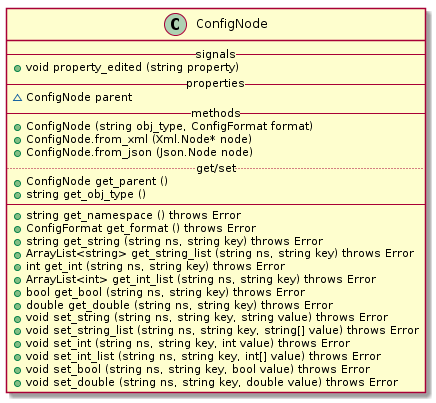
\includegraphics{figures/design/class/core/config-node}
        \end{figure}

      \emph{DcsConfig}

        \begin{figure}[H]
          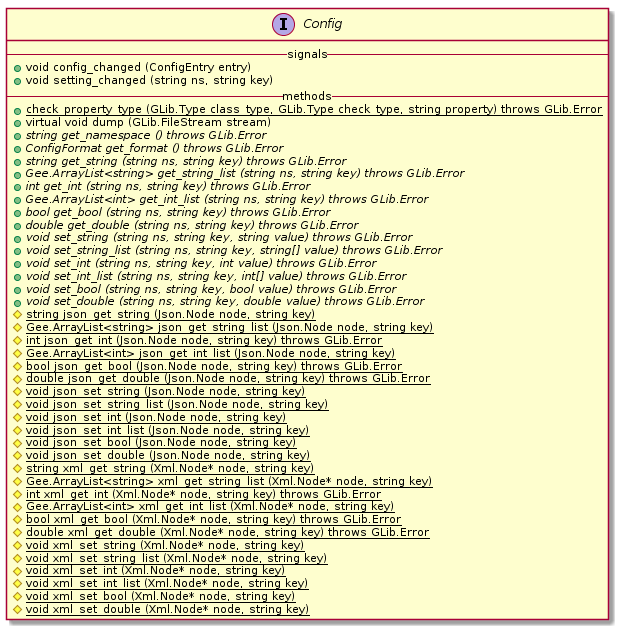
\includegraphics{figures/design/class/core/config}
        \end{figure}

      \emph{DcsContainer}

        \begin{figure}[H]
          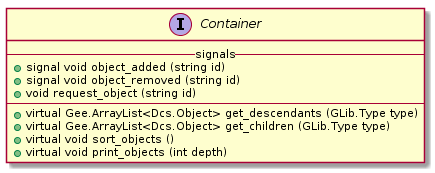
\includegraphics{figures/design/class/core/container}
        \end{figure}

      \emph{DcsController}

        \begin{figure}[H]
          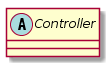
\includegraphics{figures/design/class/core/controller}
        \end{figure}

      \emph{DcsDataSeries}

        \begin{figure}[H]
          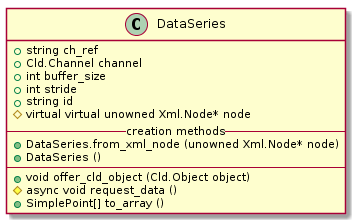
\includegraphics{figures/design/class/core/dataseries}
        \end{figure}

      \emph{DcsDBusInterface}

        \begin{figure}[H]
          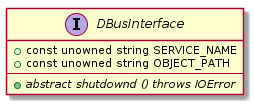
\includegraphics{figures/design/class/core/dbus-interface}
        \end{figure}

      \emph{DcsFactor}

        \begin{figure}[H]
          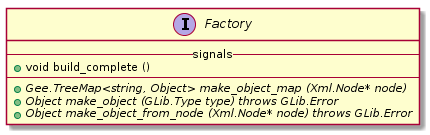
\includegraphics{figures/design/class/core/factory}
        \end{figure}

      \emph{DcsMessage}

        \begin{figure}[H]
          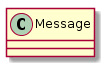
\includegraphics{figures/design/class/core/message}
        \end{figure}

      \emph{DcsMetaConfig}

        \begin{figure}[H]
          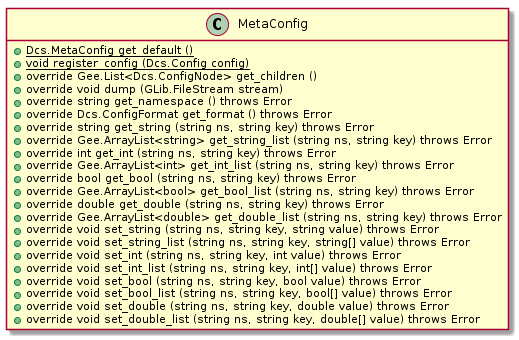
\includegraphics{figures/design/class/core/meta-config}
        \end{figure}

      \emph{DcsMetaFactory}

        \begin{figure}[H]
          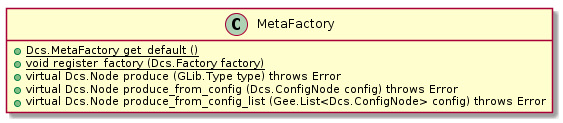
\includegraphics{figures/design/class/core/meta-factory}
        \end{figure}

      \emph{DcsModel}

        \begin{figure}[H]
          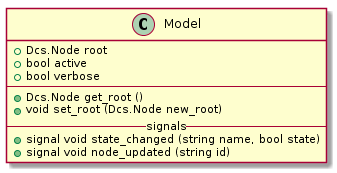
\includegraphics{figures/design/class/core/model}
        \end{figure}

      \emph{DcsNode}

        \begin{figure}[H]
          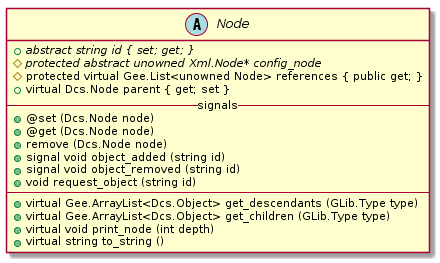
\includegraphics{figures/design/class/core/node}
        \end{figure}

      \emph{DcsObject}

        \begin{figure}[H]
          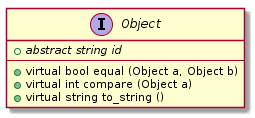
\includegraphics{figures/design/class/core/object}
        \end{figure}

      \emph{DcsPluginExtension}

        \begin{figure}[H]
          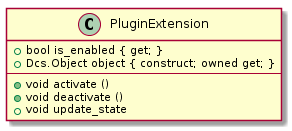
\includegraphics{figures/design/class/core/plugin-extension}
        \end{figure}

      \emph{DcsPluginInformation}

        \begin{figure}[H]
          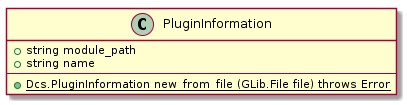
\includegraphics{figures/design/class/core/plugin-information}
        \end{figure}

      \emph{DcsPluginManager}

        \begin{figure}[H]
          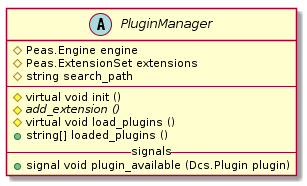
\includegraphics{figures/design/class/core/plugin-manager}
        \end{figure}

      \emph{DcsPlugin}

        \begin{figure}[H]
          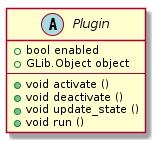
\includegraphics{figures/design/class/core/plugin}
        \end{figure}

      \emph{Point}

        \begin{figure}[H]
          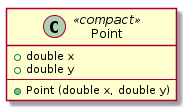
\includegraphics{figures/design/class/core/point}
        \end{figure}

      \emph{DcsRefContainer}

        \begin{figure}[H]
          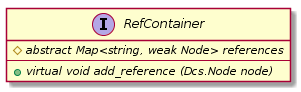
\includegraphics{figures/design/class/core/ref-container}
        \end{figure}

      \emph{DcsRefLinker}

        \begin{figure}[H]
          \includegraphics{figures/design/class/core/ref-linker}
        \end{figure}

      \emph{DcsSerializable}

        \begin{figure}[H]
          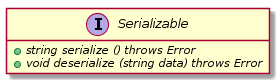
\includegraphics{figures/design/class/core/serializable}
        \end{figure}

      \emph{DcsSyslog}

        \begin{figure}[H]
          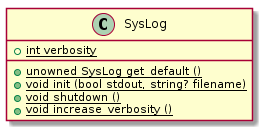
\includegraphics{figures/design/class/core/syslog}
        \end{figure}

      \emph{DcsView}

        \begin{figure}[H]
          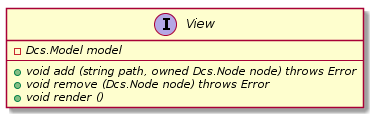
\includegraphics{figures/design/class/core/view}
        \end{figure}

    \subsubsection{Data Acquisition Library}\label{sec:dsg-classes-daq}

      \emph{DcsDaqDeviceManager}

        \begin{figure}[H]
          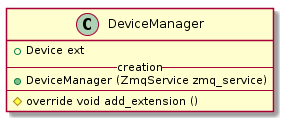
\includegraphics{figures/design/class/daq/device-manager}
        \end{figure}

      \emph{DcsDaqDevice}

        \begin{figure}[H]
          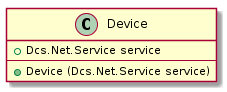
\includegraphics{figures/design/class/daq/device}
        \end{figure}

      \emph{DcsDaqFactory}

        \begin{figure}[H]
          \includegraphics{figures/design/class/daq/}
        \end{figure}

    \subsubsection{Data Logging Library}\label{sec:dsg-classes-log}

      \emph{DcsLogBackenManager}

        \begin{figure}[H]
          \includegraphics{figures/design/class/log/backend-managerd}
        \end{figure}

      \emph{DcsLogBackend}

        \begin{figure}[H]
          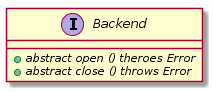
\includegraphics{figures/design/class/log/backend}
        \end{figure}

      \emph{DcsLogBackendProxy}

        \begin{figure}[H]
          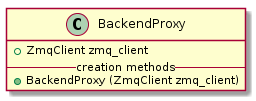
\includegraphics{figures/design/class/log/backend-proxy}
        \end{figure}

      \emph{DcsLogFactory}

        \begin{figure}[H]
          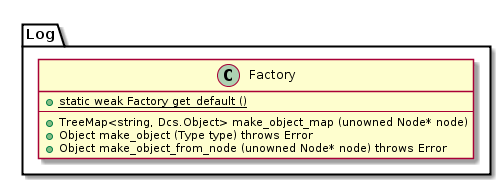
\includegraphics{figures/design/class/log/factory}
        \end{figure}

    \subsubsection{Networking Library}\label{sec:dsg-classes-net}

      \emph{DcsNetFactory}

        \begin{figure}[H]
          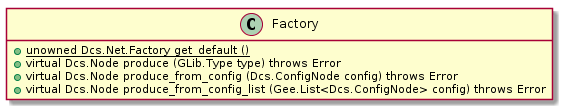
\includegraphics{figures/design/class/net/factory}
        \end{figure}

      \emph{DcsNetRestService}

        \begin{figure}[H]
          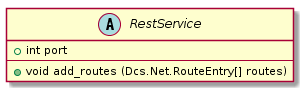
\includegraphics{figures/design/class/net/rest-service}
        \end{figure}

      \emph{DcsNetPublish}

        \begin{figure}[H]
          \includegraphics{figures/design/class/net/publish}
        \end{figure}

      \emph{DcsNetSubscribe}

        \begin{figure}[H]
          \includegraphics{figures/design/class/net/subscribe}
        \end{figure}

      \emph{DcsNetRequest}

        \begin{figure}[H]
          \includegraphics{figures/design/class/net/request}
        \end{figure}

      \emph{DcsNetReply}

        \begin{figure}[H]
          \includegraphics{figures/design/class/net/reply}
        \end{figure}

  \subsection{Class Diagrams}\label{sec:dsg-class-dia}

  \subsection{Sequence Diagrams}\label{sec:dsg-sequence}
